\section{Analisi dei requisiti} 
\subsection{Descrizione}
Si vuole realizzare una base di dati che gestisca in maniera efficiente le informazioni relative all’organizzazione del ristorante “La Sofia” a Padova. \newline
In particolare si vogliono conoscere i dati relativi a: provviste nel magazzino e nella cantina, contabilità (entrate ed uscite), dipendenti, turni di lavoro e prenotazioni effettuate per il locale. \medskip \\
Di ciascun \textbf{prodotto} si vuole sapere:
\begin{itemize}
    \item Codice idenficativo progessivo numerico
    \item Nome
    \item Quantità presente nel magazzino
    \item Prezzo
    \item Fornitore
\end{itemize}
Un prodotto può essere o un cibo o una bevanda. \\
Un cibo può essere fresco, a lunga conservazione o surgelato. Per ogni cibo si vuole sapere anche la data di scadenza. \\
Una bevanda, di cui si vuole sapere la marca, può essere non alcolica o alcolica. Gli alcolici si dividono in vini e superalcolici. Per entrambi si vuole sapere sia l’annata che il tipo. \\
Per i prodotti da frigo, o freschi, si vuole inoltre conoscere la data di scadenza. \medskip \\
Per quanto riguarda i rifornimenti, per ogni \textbf{fornitore} si vuole sapere:
\begin{itemize}
    \item Partita IVA che lo identifica univocamente
    \item Nome azienda
    \item Recapito telefonico
\end{itemize}
Riguardo alla contabilità, di ogni \textbf{uscita ed entrata} si vuole sapere:
\begin{itemize}
    \item Codice identificativo progessivo numerico
    \item Costo %valore
    \item Data
\end{itemize}
La contabilità comprende sia le entrate che le uscite. \\
Di ogni uscita deve essere specificata anche la motivazione o causale che ha generato il costo. \\
Ogni uscita può corrispondere o all'acquisto di un prodotto o al salario di un dipendente. \\
Ogni entrata corrisponde ad un eventuale incasso derivante da un'ordine. \medskip \\
Di ogni \textbf{Ordine} si vuole sapere:
\begin{itemize}
    \item Numero tavolo 
    \item Numero di persone 
    \item Cameriere che serve l'ordine
    \item Conto totale
    \item Giorno
    \item Ora
\end{itemize}
Ogni ordine è identificato dal numero del tavolo, il giorno e l'ora. \\
Ogni ordine è preso e servito da un cameriere. \medskip \\
Per le \textbf{prenotazioni} effettuate per il locale si vuole sapere:
\begin{itemize}
    \item Numero del tavolo
    \item Giorno della prenotazione
    \item Ora della prenotazione
    \item Nome del prenotante
    \item Numero di persone al tavolo
\end{itemize}
Ogni prenotazione è identificata univocamente da giorno, ora e numero del tavolo. \\
Il numero di persone per tavolo non può superare il numero di coperti disponibili per quel tavolo. \medskip \\ 
Di ogni \textbf{Tavolo} si vuole sapere:
\begin{itemize}
    \item Numero del tavolo che lo identifica univocamente
    \item Quantità di coperti disponibili
\end{itemize}
Riguardo al \textbf{personale} invece si vuole sapere:
\begin{itemize}
    \item Codice fiscale, che identifica ogni dipendente univocamente
    \item Nome 
    \item Cognome 
    \item Giorno libero
    \item Stipendio
\end{itemize}
Il personale si divide in cuochi, sommelier o camerieri.\\
Il giorno di riposo non può corrispondere ad un giorno nei turni di lavoro. \\
Solo i camerieri possono servire ai tavoli. \medskip \\
Riguardo ai \textbf{turni di lavoro} all’interno del locale, si vuole sapere:
\begin{itemize}
    \item Codice del dipendente
    \item Giorno, che lo identifica univocamente
\end{itemize}
Ogni turno di lavoro comprende l'intera giornata, senza distinzione tra pranzo e cena.

\subsection{Glossario dei termini}
\begin{longtable}{p{2.5cm} p{6cm} p{2cm} p{5.5cm}}
    \toprule
    \textbf{Termine} & \textbf{Descrizione} & \textbf{Sinonimi} & \textbf{Collegamenti}\\ \midrule
    Prodotto & Cibo o bevanda presente nel magazzino & Provviste & Fornitore, Contabilità \\ \midrule
    Fornitore & Azienda fornitrice di prodotti & Azienda & Prodotto \\ \midrule
    Contabilità & Uscite ed entrate del ristorante & Spesa & Prodotto, Ordine, Personale \\ \midrule
    Ordine & Ordine effettuato dai clienti ad un determinato tavolo & & Contabilità, Personale, Tavolo \\ \midrule
    Prenotazione & Prenotazione per un tavolo del ristorante & & Tavolo \\ \midrule
    Tavolo & Tavolo & & Prenotazione, Ordine\\ \midrule
    Personale & Dipendenti a servizio del locale & Dipendente & Contabilità, Ordine, Turni\\ \midrule
    Turni & Turni lavorativi dei dipendenti & & Personale	\\ \midrule
\end{longtable}

\subsection{Operazioni}
\begin{description}
    \item [Operazione 1:] inserimento di un nuovo prodotto.
    \item [Operazione 2:] modificare la quantità di un prodotto.
    \item [Operazione 3:] inserimento di una nuova prenotazione.
    \item [Operazione 4:] cancellazione di una prenotazione.
    \item [Operazione 5:] inserimento di un nuovo dipendente.
    \item [Operazione 6:] modifica di un turno di lavoro .
    \item [Operazione 7:] stampare il codice, nome e quantità di tutti i prodotti che sono cibi e che scadono entro il 28 febbraio 2019, che inoltre iniziano con la R, ordinati in modo decrescente.
    \item [Operazione 8:] stampa il codice, il nome, la marca e l’annata di tutti i vini con annata risalente a massimo il 2008 e prezzo inferiore a 20 euro ordinati per prezzo crescente.
    \item [Operazione 9:] stampa il numero dei tavoli liberi nel giorno 20/02/2019 che non hanno 3 o 4 coperti.
    \item [Operazione 10:] stampa nome e cognome di tutti i dipendenti di turno il martedì.
    \item [Operazione 11:] calcola il guadagno mensile dato dalla differenza tra la somma delle entrate e la somma delle uscite.
    \item [Operazione 12:] trova il cameriere che effettua più ordini in media al giorno per decidere se promuoverlo o no.
\end{description}

\subsection{Strutturazione dei requisiti} 
\begin{longtable}{|p{17cm}|}
    \hline
    \textbf{Frasi di carattere generale} \\ \hline
    Si vuole realizzare una base di dati che gestisca in maniera efficiente le informazioni relative all’organizzazione del ristorante “La Sofia” a Padova. In particolare si vogliono conoscere i dati relativi a provviste nel magazzino e nella cantina, contabilità (entrate ed uscite), dipendenti, turni di lavoro e prenotazioni effettuate per il locale. \\ \hline
\end{longtable}

\begin{longtable}{|p{ 17cm}|}
    \hline
    \textbf{Frasi relative a prodotto} \\ \hline
    Ogni prodotto ha: un codice idenficativo progessivo numerico, un nome, una quantità, un prezzo ed un fornitore.\\
    Un prodotto può essere o un cibo o una bevanda.
    Un cibo può essere fresco, a lunga conservazione o surgelato.
    Una bevanda, di cui si vuole sapere la marca, può essere non alcolica o alcolica. Gli
    alcolici si dividono in vini e superalcolici. Per entrambi si vuole sapere sia l’annata che
    il tipo.
    Per i vini i tipi possono essere rosso, bianco fermo, rosè, frizzante, passito. Per i
    superalcolici i tipi sono grappa, amaro, whisky, rum, aperol.
    Per i prodotti da frigo, o freschi, si vuole inoltre conoscere la data di scadenza.\\ \hline
\end{longtable}

\begin{longtable}{|p{17cm}|}
    \hline
    \textbf{Frasi relative a fornitore} \\ \hline
    Ogni fornitore ha: un codice dell'azienda corrispondente alla Partita IVA che lo identifica univocamente, un nome ed un recapito telefonico.\\
    Ogni fornitore vende uno o più prodotti al ristorante.
    \\ \hline
\end{longtable}

\begin{longtable}{|p{17cm}|}
    \hline
    \textbf{Frasi relative a contabilità} \\ \hline
    Ogni entrata ed uscita ha: un codice idenficativo progressivo numerico, un costo ed una data.\\
    La contabilità comprende sia le entrate che le uscite.
    Di ogni uscita deve essere specificata anche la motivazione o causale che ha generato
    il costo.
    Ogni uscita può corrispondere o all’acquisto di un prodotto o al salario di un dipendente.
    Ogni entrata corrisponde ad un eventuale incasso derivante da un’ordine.
    \\ \hline
\end{longtable}

\begin{longtable}{|p{17 cm}|}
    \hline
    \textbf{Frasi relative a ordine} \\ \hline
    Ogni ordine ha: un numero corrispondente al tavolo, il numero di persone per tavolo il cameriere che serve al tavolo, un totale, il giorno e l'ora. \\
    Ogni ordine è identificato dal numero del tavolo, il giorno e l’ora.
    Ogni ordine è preso e servito da un cameriere.
    \\ \hline
\end{longtable}

\begin{longtable}{|p{17 cm}|}
    \hline
    \textbf{Frasi relative a prenotazione} \\ \hline
    Ogni prenotazione ha: un nome del cliente prenotante, il giorno della prenotazione, l'ora della prenotazione, un numero di persone al tavolo. 
    Ogni prenotazione è identificata univocamente da giorno, ora e numero del tavolo.
    Il numero di persone per tavolo non può superare il numero di coperti disponibili per
    quel tavolo.
    \\ \hline
\end{longtable}

\begin{longtable}{|p{17 cm}|}
    \hline
    \textbf{Frasi relative a tavolo} \\ \hline
    Ogni tavolo ha: un numero del tavolo che lo identifica univocamente, una quantità di coperti. \\
    Ad un tavolo può corrispondere una prenotazione. 
    Per ogni tavolo può corrispondere un ordine.
    \\ \hline
\end{longtable}
\begin{longtable}{|p{17 cm}|}
    \hline
    \textbf{Frasi relative a personale} \\ \hline
    Ogni dipendente ha: un codice fiscale, che identifica ogni dipendente univocamente, un nome ed un cognome, il giorno di riposo, uno stipendio. \\
    Il personale si divide in cuochi, sommelier o camerieri.
    Ogni dipendente non può coprire un turno di lavoro nel suo giorno libero.
    Solo i camerieri possono servire ai tavoli.
    \\ \hline
\end{longtable}
\begin{longtable}{|p{17 cm}|}
    \hline
    \textbf{Frasi relative a turni di lavoro} \\ \hline
    Ogni turno di lavoro ha: un codice del dipendente ed un giorno. \\
    Ogni turno di lavoro viene identificato univocamente dal giorno.
    Ogni turno di lavoro comprende l’intera giornata, senza distinzione tra pranzo e cena.
    \\ \hline
\end{longtable}

\section{Schema concettuale} %Schema ER
%Immagine
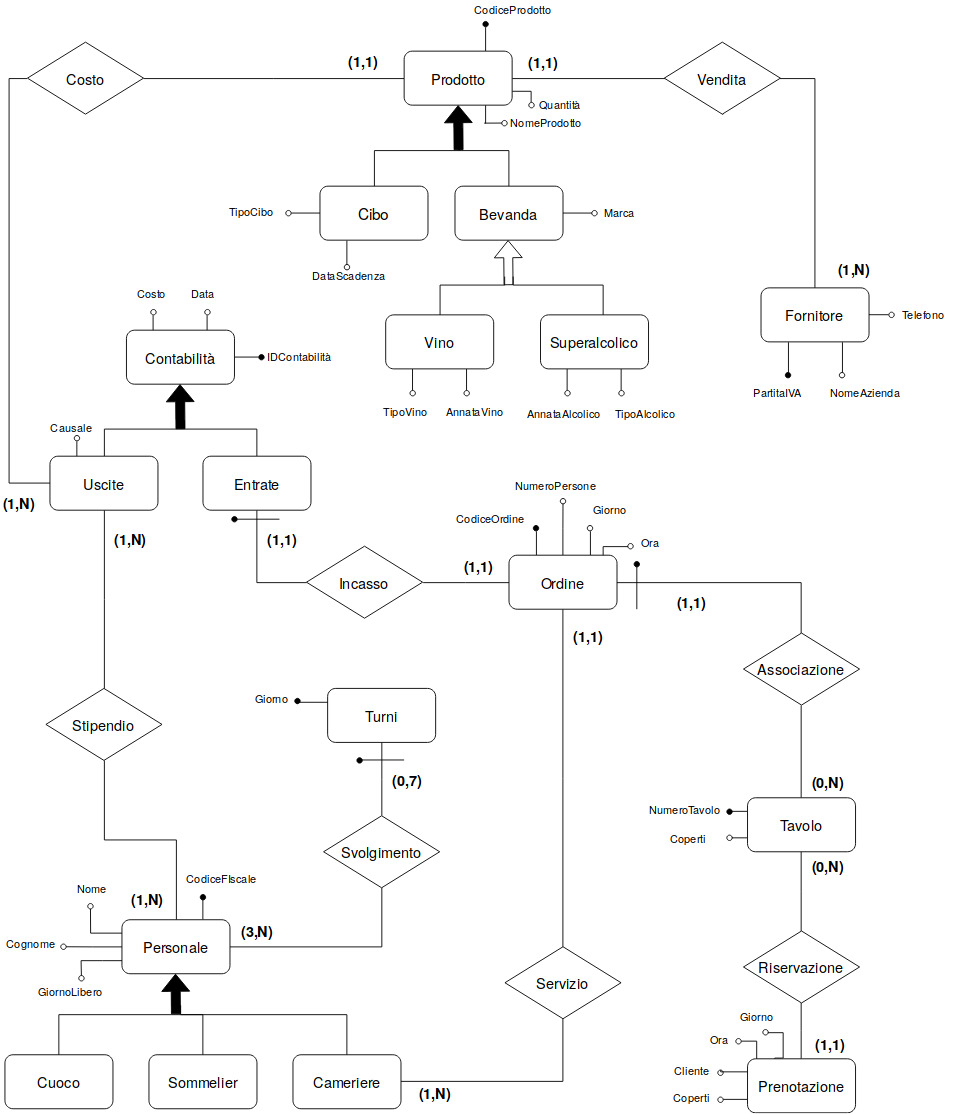
\includegraphics[width=1\textwidth]{doc/schema}
\subsection{Dizionario dei dati}
\textbf{Regole di vincolo} 
\begin{itemize}
    \item Un dipendente non può svolgere più di 6 turni a settimana.
    \item Un cliente non può prenotare un tavolo già prenotato.
    \item Il numero del tavolo deve essere compreso tra 1 e 35.
    \item La quantità del prodotto non può essere negativa.
\end{itemize}

\textbf{Lista delle entità}
\begin{longtable}{p{2.5cm} p{5.5cm} p{5.5cm} p{2.5cm}}
    \toprule
    \textbf{Entità} & \textbf{Descrizione} &   \textbf{Attributi} & \textbf{Identificatore}\\ \midrule
    Prodotto & Provvista del magazzino & CodiceProd, NomeProdotto, Quantità & CodiceProd\\ \midrule
    Cibo & Prodotto commestibile & Eredita da Prodotto, TipoCibo, DataScadenza & CodiceProd \\ \midrule
    Bevanda	& Prodotto da bere & Eredita da prodotto, Marca & CodiceProd\\ \midrule
    Vino & Bevanda alcolica a base di uva & Eredita da bevanda, AnnataVino, TipoVino & CodiceProd \\ \midrule
    Superalcolico & Bevanda con grado alcolico elevato & Eredita da Bevanda, TipoAlcolico, AnnataAlcolico & CodiceProd \\ \midrule
    Fornitore & Azienda fornitrice di prodotti & PartitaIva, NomeAzienda, Telefono & PartitaIva \\ \midrule
    Contabilità & Gestione del denaro del locale & CodiceCont, Costo, Data &CodiceCont \\ \midrule
    Entrata & Entrata di denaro del ristorante & Eredita da contabilità & CodiceCont \\ \midrule
    Uscita & Uscita di denaro dal ristorante & Eredita da contabilità, Causale & CodiceCont \\ \midrule
    Ordine & Ordine effettuato per un determinato tavolo & NumeroTavolo, NumeroPersone, Giorno, Ora & NumeroTavolo, Giorno, Ora\\ \midrule
    Prenotazione & Prenotazione per un tavolo del ristorante & NumeroTavolo, Giorno, Ora, NumeroCoperti, Cliente & Numerotavolo, Giorno, Ora \\ \midrule
    Tavolo & Tavolo presente nel locale & NumeroTavolo, Coperti & NumeroTavolo\\ \midrule
    Personale & Insieme dei dipendenti del locale & CodiceFiscale, Nome, Cognome, GiornoLibero & CodiceFiscale\\ \midrule
    Cuoco & Dipendente addetto alla cucina & Eredita da personale & CodiceFiscale\\ \midrule
    Sommelier & Dipendente addetto alla mescita degli alcolici & Eredita da personale & CodiceFiscale\\ \midrule
    Cameriere & Dipendente che serve ai tavoli & Eredita da personale & CodiceFiscale\\ \midrule
    Turno & Turno di lavoro & Giorno & Giorno\\ 
    \bottomrule	
\end{longtable}
\textbf{Lista delle relazioni} 
\begin{longtable}{p{2.5cm} p{7.5cm} p{3.5cm} p{2.5cm}}
    \midrule
    \textbf{Relazione} & \textbf{Descrizione} & \textbf{Cardinalità} & \textbf{Attributi} \\ \midrule
    Vendita & Associa il prodotto al suo fornitore & Prodotto(1,1) \newline Fornitore(1,N) &  \\ \midrule
    Costo & Associa il prezzo del prodotto all'uscita di denaro & Prodotto(1,1) \newline Uscita(1,N) & \\ \midrule
    Incasso & Associa l'ordine all'entrata di denaro & Ordine(1,1) \newline Entrata(1,1) &  \\ \midrule
    Associazione & Associa l'ordine al tavolo & Ordine(1,1) \newline Tavolo(0,N) &  \\ \midrule
    Riservazione & Associa il tavolo alla prenotazione & Tavolo(0,N) \newline Prenotazione(1,1) &  \\ \midrule
    Servizio & Associa l'ordine al cameriere & Ordine(1,1) \newline Cameriere(1,N) & \\ \midrule
    Svolgimento & Associa il dipendente al turno di lavoro & Personale(3,N) \newline Turno(0,7) & \\ \midrule
    Stipendio & Associa lo stipendio del dipendente all'uscita del ristorante & Dipendente(1,N) \newline Uscita(1,N) &  \\ \bottomrule
\end{longtable}

